%% Solution of part 1
\subsubsection*{1.A}
Since the input signal $r_k$ is white, the $R$ matrix only has non-zero entries in its main diagonal:

\begin{equation}
R = \mathrm{diag}([1, \sigma^2_r, \ldots, \sigma^2_r]) \implies \mathrm{tr}(R) = (L+1)\sigma^2_r + 1,
\end{equation} 
where the first entry is 1 because the bias weight input is always $+1$. Therefore,
\begin{equation}
\mu = 0.01\frac{1}{\mathrm{tr}(R)} = \frac{0.01}{(L+1)\sigma^2_r + 1} = 2.439\times 10^{-4}.
\end{equation}

\subsubsection*{1.B}
The Matlab code to calculate the learning curve is included below. Figure~\ref{fig:part1-learning-curve} shows the learning curve averaged over 100 independent input realizations, and  Figure~\ref{fig:part1-weights} shows the converged weight vector. Note that the bias weight value is very significant.

\FloatBarrier
\begin{figure}[h!]
	\centering
	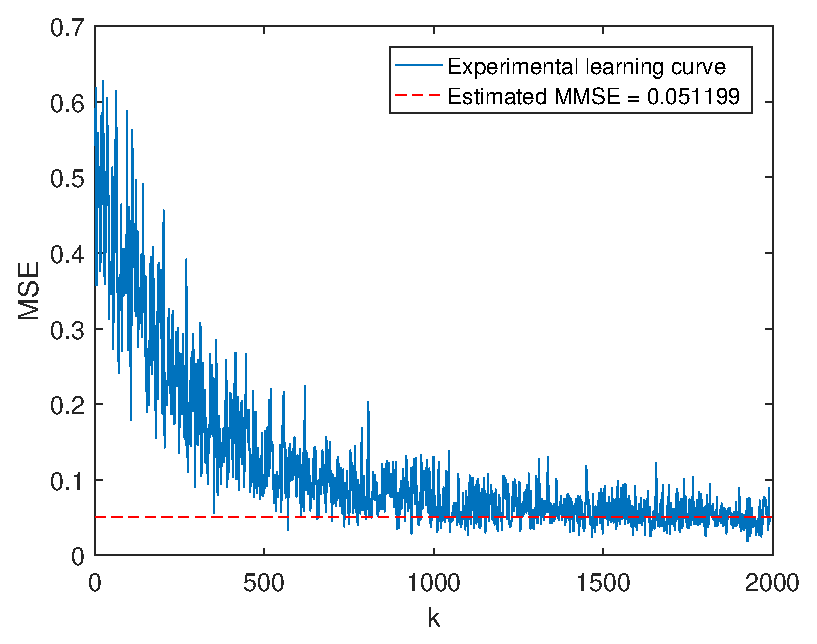
\includegraphics[scale=0.8]{part1_learning_curve.eps}
	\caption{Experimental learning curve for nonlinear plant indemnification using a linear filter. The learning curve was averaged 100 times.}
	\label{fig:part1-learning-curve}
\end{figure}
\FloatBarrier

\FloatBarrier
\begin{figure}[h!]
	\centering
	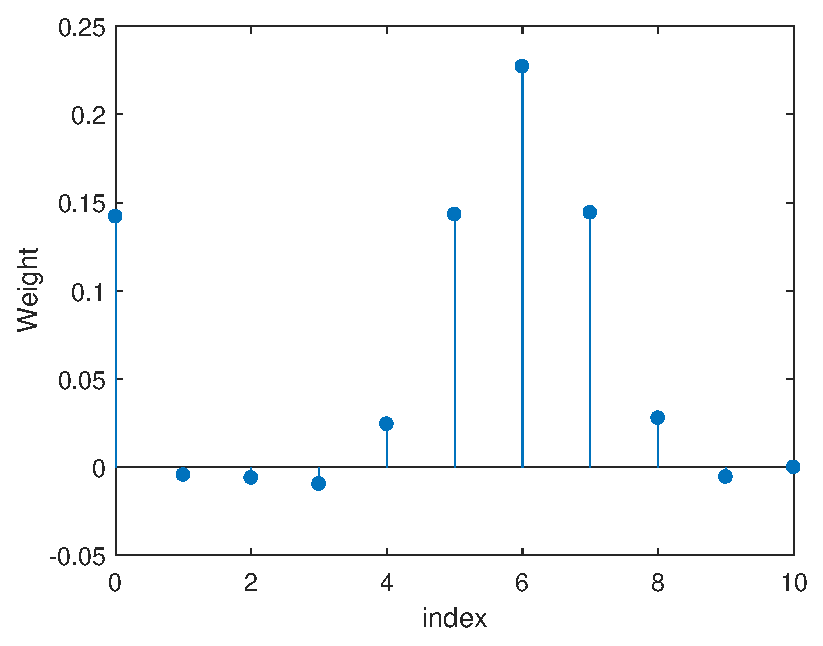
\includegraphics[scale=0.8]{part1_weights.eps}
	\caption{Weight vector after convergence.}
	\label{fig:part1-weights}
\end{figure}
\FloatBarrier

\subsubsection*{1.C}
As shown in Figure~\ref{fig:part1-learning-curve}, the MMSE estimated using the last 200 samples was equal to $\approx 0.051$.

\subsubsection*{1.D}
As discussed in class, the convergence time of the learning curve depends on the eigenvalues of the matrix $R$. Since $R$ is a diagonal matrix, its eigenvalues are equal to the entries in the main diagonal:
\begin{equation}
\lambda_1 = 1, \qquad \lambda_2 = \ldots = \lambda_{L+2} = \sigma_r^2.
\end{equation}

The time constants $\tau_n = 1/2\mu\lambda_n$ are therefore
\begin{equation}
\tau_1 = \frac{1}{2\mu}, \qquad \tau_2 = \ldots = \tau_{L+2} = \frac{1}{2\mu\sigma_r^2}.
\end{equation}

The learning curve has two modes. One due to the bias weight, and another due to the signal inputs. The slowest mode will determine the convergence time of the learning curve. 

In the first case, when $\sigma_r^2 = 4$, the slowest mode is due to the bias weight since $\tau_n < \tau_1, n > 1$. Therefore, the slowest time constant is $\tau_1 = 2050$. The approximate number of iterations for convergence is given by $(T_{mse})_1 = 0.5\tau_1 = 1025$, which we can verify this from Figure~\ref{fig:part1-learning-curve}.

When, $\sigma_r^2$ is made small. The mode due to the signal inputs will become the slowest one. And since we're assuming that $(L+1)\sigma_r^2 << 1$, the time constant due to the input signals is inversely proportional to the signal variance $\sigma_r^2$, as $\mu\approx 0.01$. Thus, the time constant is $\tau_n = 50/\sigma_r^2 >> 2050$. Therefore, the convergence time of the learning curve increases as we decrease the input signal power.

As for the MMSE, the MMSE is smaller for smaller $\sigma_r^2$. When the input signal is small enough to make the plant nonlinearity negligible, the plant is essentially the linear filter $\frac{1}{2}H_1(z)H_2(z)$, which is an FIR filter with 11 taps. The factor of $\frac{1}{2}$ appears because $g(x) \approx x/2, x \to 0$, which follows from the Taylor series expansion of $g(x)$. The adaptive filter has 10 taps plus the bias weight, and thus it could model the plant not perfectly, but very well. 

\subsubsection*{1.E}
The Matlab code is the same as for part (B) and it is shown below. The output of the plant is compared to the output of the adaptive filter in Figure~\ref{fig:part1-test}.

\FloatBarrier
\begin{figure}[h!]
	\centering
	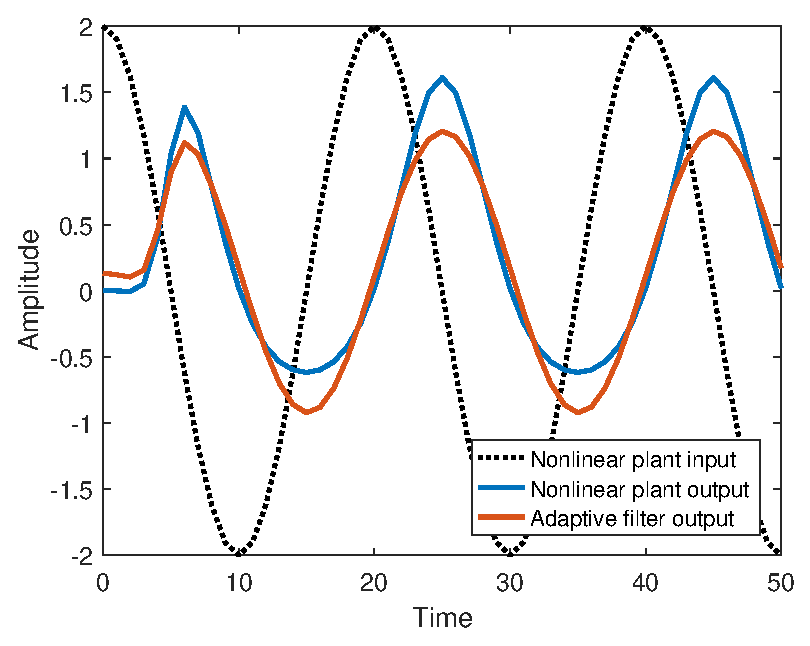
\includegraphics[scale=0.8]{part1_test.eps}
	\caption{Test of the adaptive filter after convergence with a sinusoidal signal. During the first $L+1$ samples, the filter was being initialized.}
	\label{fig:part1-test}
\end{figure}
\FloatBarrier
